% Poster of the final project: 70 x 100 cm, one page.
% The figures come from poster/poster_figures.py. Compile twice with lualatex.
\documentclass{article}
\usepackage[paperwidth=700mm, paperheight=1000mm, margin=0mm]{geometry}
\usepackage{fontspec}
\usepackage{unicode-math}
\setmainfont{FiraSans}[
  Extension = .otf,
  UprightFont = *-Regular,
  BoldFont = *-SemiBold,
  ItalicFont = *-Italic,
  BoldItalicFont = *-SemiBoldItalic,
]
\setmathfont{FiraMath-Regular.otf}
\usepackage{xcolor}
\usepackage{graphicx}
\usepackage{qrcode}
\usepackage{tikz}
\usetikzlibrary{arrows.meta, calc, positioning}

\definecolor{ink}{HTML}{1D2433}
\definecolor{ink2}{HTML}{4A5160}
\definecolor{soft}{HTML}{8A90A0}
\definecolor{rule}{HTML}{DCDCD6}
\definecolor{input}{HTML}{B5604E}
\definecolor{method}{HTML}{2A78D6}
\definecolor{faired}{HTML}{EB6834}
\definecolor{symmetry}{HTML}{1BAF7A}
\definecolor{original}{HTML}{7E848A}
\definecolor{paper}{HTML}{EEF0F3}

\pagestyle{empty}
\setlength{\parindent}{0pt}
\setlength{\parskip}{0pt}
\hyphenpenalty=10000
\exhyphenpenalty=10000
\color{ink}

\newcommand{\bodytext}{\fontsize{27}{35}\selectfont}
\newcommand{\smalltext}{\fontsize{22}{28}\selectfont}
\newcommand{\tinytext}{\fontsize{18}{23}\selectfont}

% Section heading: number in a circle and title.
\newcommand{\heading}[2]{%
  {\fontsize{44}{50}\selectfont
   \tikz[baseline=(n.base)]\node[circle, fill=ink, text=white, inner sep=0pt,
     minimum size=16mm, font=\fontsize{32}{32}\selectfont\bfseries](n){#1};%
   \hspace{5mm}\textbf{#2}\par}%
  \vspace{6mm}}

\newcommand{\bulletitem}[1]{%
  \hangindent=7mm\hangafter=1
  \makebox[7mm][l]{\textcolor{soft}{\textbullet}}#1\par\vspace{2.5mm}}

% Entry of the reference list, with a hanging indent.
\newcommand{\bib}[1]{\par\vspace{0.6mm}\hangindent=9mm\hangafter=1\makebox[9mm][l]{[#1]}}

% Label of a figure column, centered in a given width.
\newcommand{\collabel}[3]{\makebox[#1][c]{\textcolor{#2}{\bfseries #3}}}

% TikZ sets \spaceskip in em of the font size of the node: this restores the spacing of each font.
\newcommand{\resetspaces}{\spaceskip=0pt\xspaceskip=0pt\relax}

% Absolute placement: \placeblock{x}{y}{width}{content}, in mm from the upper left
% corner. Without the align option of TikZ, which sets the interword space to the font
% size of the node.
\newcommand{\placeblock}[4]{%
  \node[anchor=north west, inner sep=0pt, text width=#3mm]
    at ($(current page.north west) + (#1mm, -#2mm)$) {\resetspaces\raggedright #4};}

\tikzset{
  every node/.append style={execute at begin node=\resetspaces},
  stage/.style={draw=soft, fill=paper, rounded corners=3mm, line width=1.2mm,
    minimum height=23mm, text width=47mm, align=center, inner sep=2mm,
    font=\fontsize{22}{26}\selectfont},
  own/.style={stage, line width=1.8mm, font=\fontsize{22}{26}\selectfont\bfseries},
  arrow/.style={-{Latex[length=6mm, width=6mm]}, line width=1.3mm, draw=ink2},
  note/.style={font=\fontsize{19}{23}\selectfont, text=ink2},
}

\begin{document}
\begin{tikzpicture}[remember picture, overlay]

% ---------------------------------------------------------------- header
\fill[ink] (current page.north west) rectangle ($(current page.north east) + (0, -104mm)$);
\placeblock{25}{11}{490}{%
  {\fontsize{112}{116}\selectfont\bfseries\color{white} Completing broken meshes\par}
  \vspace{7mm}
  {\fontsize{34}{43}\selectfont\color{white!78!ink}
   An extension of Jacobson, Kavan and Sorkine-Hornung (SIGGRAPH 2013) with cap
   fairing and symmetry completion\par}}
\node[anchor=north east, inner sep=0pt, text width=150mm]
  at ($(current page.north east) + (-25mm, -19mm)$) {\resetspaces\raggedleft\color{white}
  {\fontsize{40}{50}\selectfont\bfseries Lucas Allara\par}
  \vspace{5mm}
  {\fontsize{30}{40}\selectfont\color{white!78!ink}
   Computer Graphics\\ Universidad Torcuato Di Tella\\ Second semester of 2026\par}};

% ---------------------------------------------------------------- teaser
\placeblock{25}{116}{650}{%
  \fontsize{30}{36}\selectfont
  \collabel{130mm}{input}{Input}%
  \collabel{130mm}{method}{Method of [1]}%
  \collabel{130mm}{faired}{With fairing}%
  \collabel{130mm}{symmetry}{With fairing and symmetry}%
  \collabel{130mm}{original}{Original}\par
  \vspace{3mm}
  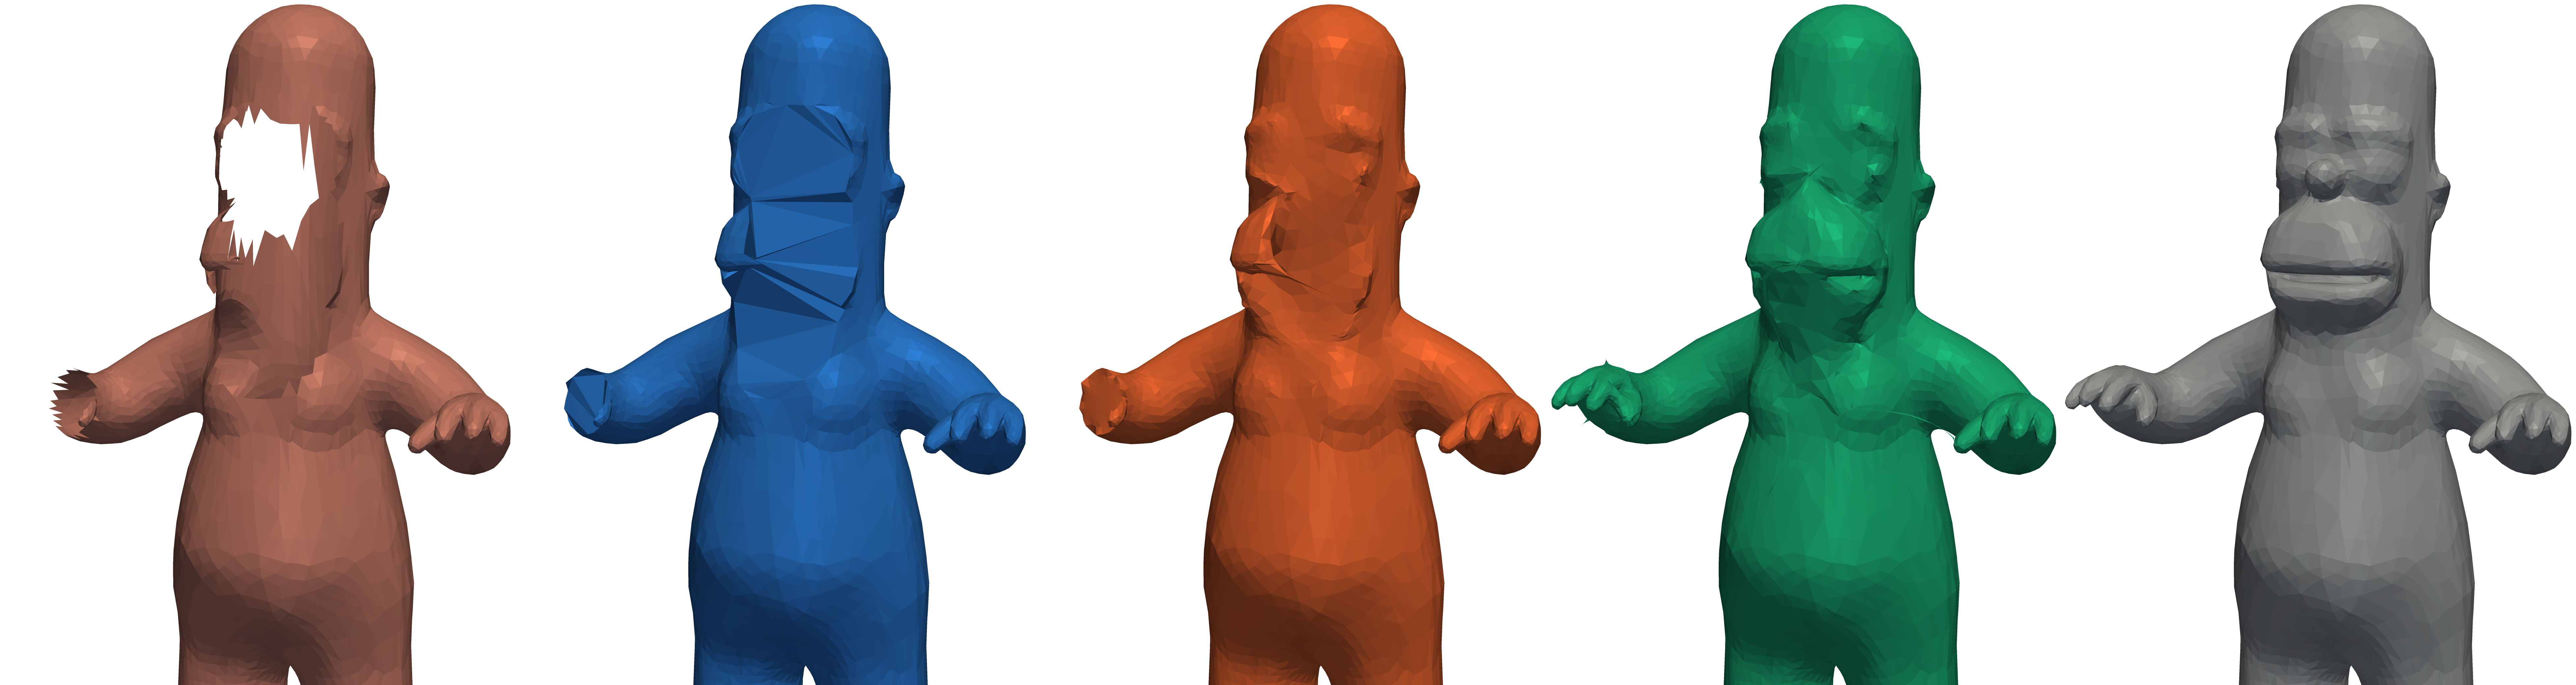
\includegraphics[width=650mm, trim=0 300 0 0, clip]{figures/teaser.png}\par}

% ---------------------------------------------------------------- 1
\placeblock{25}{293}{305}{%
  \heading{1}{Introduction}
  {\bodytext Many real meshes have holes, overlapping pieces or loose faces, and simulating
   or printing a model requires knowing which points are inside. Jacobson et al.\ [1] use the
   generalized winding number, which adds up the solid angles that the faces subtend as seen
   from \(p\).\par}
  \vspace{3mm}
  {\centering\fontsize{38}{46}\selectfont
   \(w(p) = \dfrac{1}{4\pi} \displaystyle\sum_{f} \Omega_f(p)\)\par}
  \vspace{2mm}
  {\centering
   \begin{minipage}{150mm}
     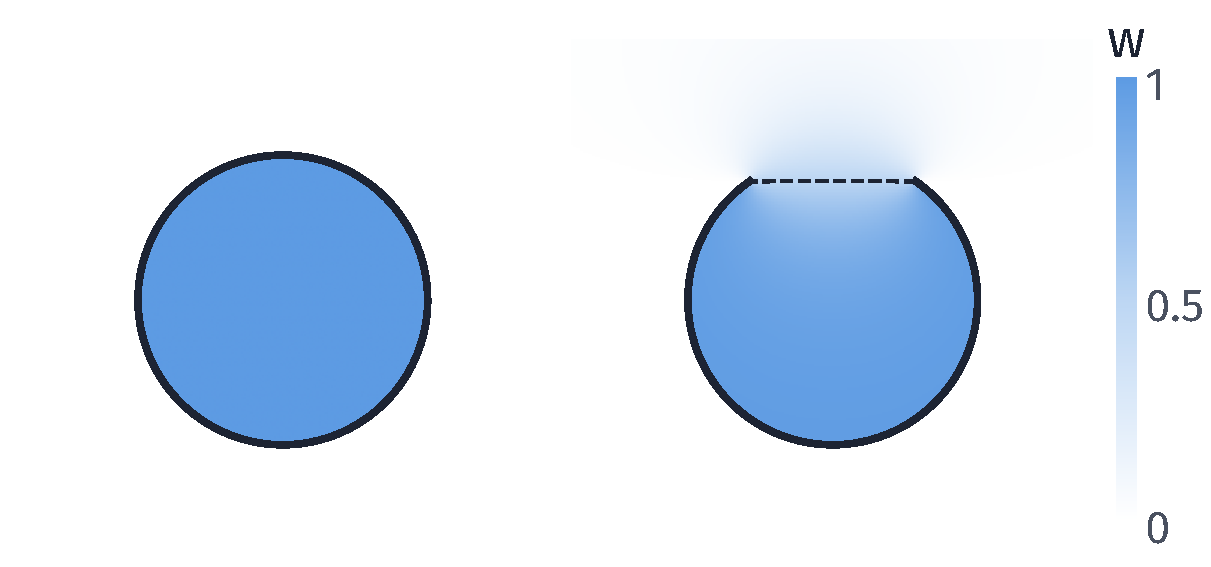
\includegraphics[width=150mm]{figures/w_cut.pdf}\par
     {\smalltext\color{ink2}
      \collabel{68mm}{ink2}{closed mesh}\collabel{68mm}{ink2}{with a hole}\par}
   \end{minipage}\par}
  \vspace{4mm}
  {\bodytext Space is tetrahedralized respecting the input faces [2], \(w\) is evaluated in
   each tetrahedron, and a graph cut chooses which ones lie inside, penalizing the separation
   of similar neighbors. Two heuristics correct the result so that the output, the boundary of
   that region, contains the input faces and is a manifold.\par}}

% ---------------------------------------------------------------- 2
\placeblock{360}{293}{315}{%
  \heading{2}{Proposal}
  {\bodytext Where surface was missing, the output of [1] is made of faces of the
   tetrahedralization, which close the hole with flat triangles and no detail. Two stages are
   added without modifying those of the method, taking ideas from the fairing of TetWild [3]
   and from symmetry completion [5].\par}
  \vspace{7mm}
  {\centering
   \begin{tikzpicture}[node distance=12mm and 11mm]
     \node[stage, text width=34mm] (e1) {Input};
     \node[stage, text width=92mm, right=of e1] (p1) {Tetrahedralization,\\\(w\) and graph cut};
     \node[own, draw=faired, fill=faired!12, text width=56mm, below=20mm of p1.south east,
       anchor=north west, xshift=11mm] (s2) {Fairing\\\(\Delta^3 x = 0\)};
     \node[stage, text width=34mm, below=20mm of e1] (e2) {Input};
     \node[stage, text width=92mm, right=of e2] (p2) {Tetrahedralization,\\\(w\) and graph cut};
     \node[stage, text width=34mm, right=36mm of s2, draw=ink, fill=white, line width=1.8mm,
       font=\fontsize{22}{26}\selectfont\bfseries] (o2) {Output};
     \node[stage, text width=34mm, draw=ink, fill=white, anchor=center] (o1)
       at (o2.center |- p1.center) {Output};
     \node[own, draw=symmetry, fill=symmetry!12, text width=54mm, anchor=north] (r)
       at ($(p2.south)!0.5!(s2.south) + (0, -14mm)$) {Symmetry\\completion};
     \node[note, anchor=south west, inner sep=0pt] at ($(e1.north west) + (0, 3mm)$)
       {\bfseries Method of [1]};
     \node[note, anchor=south west, inner sep=0pt] at ($(e2.north west) + (0, 3mm)$)
       {\bfseries Proposal};
     \draw[arrow] (e1) -- (p1);
     \draw[arrow] (p1) -- (o1);
     \draw[arrow] (e2) -- (p2);
     \draw[arrow] (p2) -- (s2);
     \draw[arrow] (s2) -- node[note, above=1mm] {2nd pass} (o2);
     \draw[arrow, draw=symmetry] (s2.south) |- node[note, pos=0.3, right=2mm, text=symmetry]
       {1st pass} (r.east);
     \draw[arrow, draw=symmetry] (r.west) -| node[note, pos=0.75, left=2mm, text=symmetry,
       align=right] {2nd pass, with the\\mirrored faces} (p2.south);
   \end{tikzpicture}\par}
  \vspace{9mm}
  \begin{minipage}[t]{150mm}\resetspaces\raggedright
    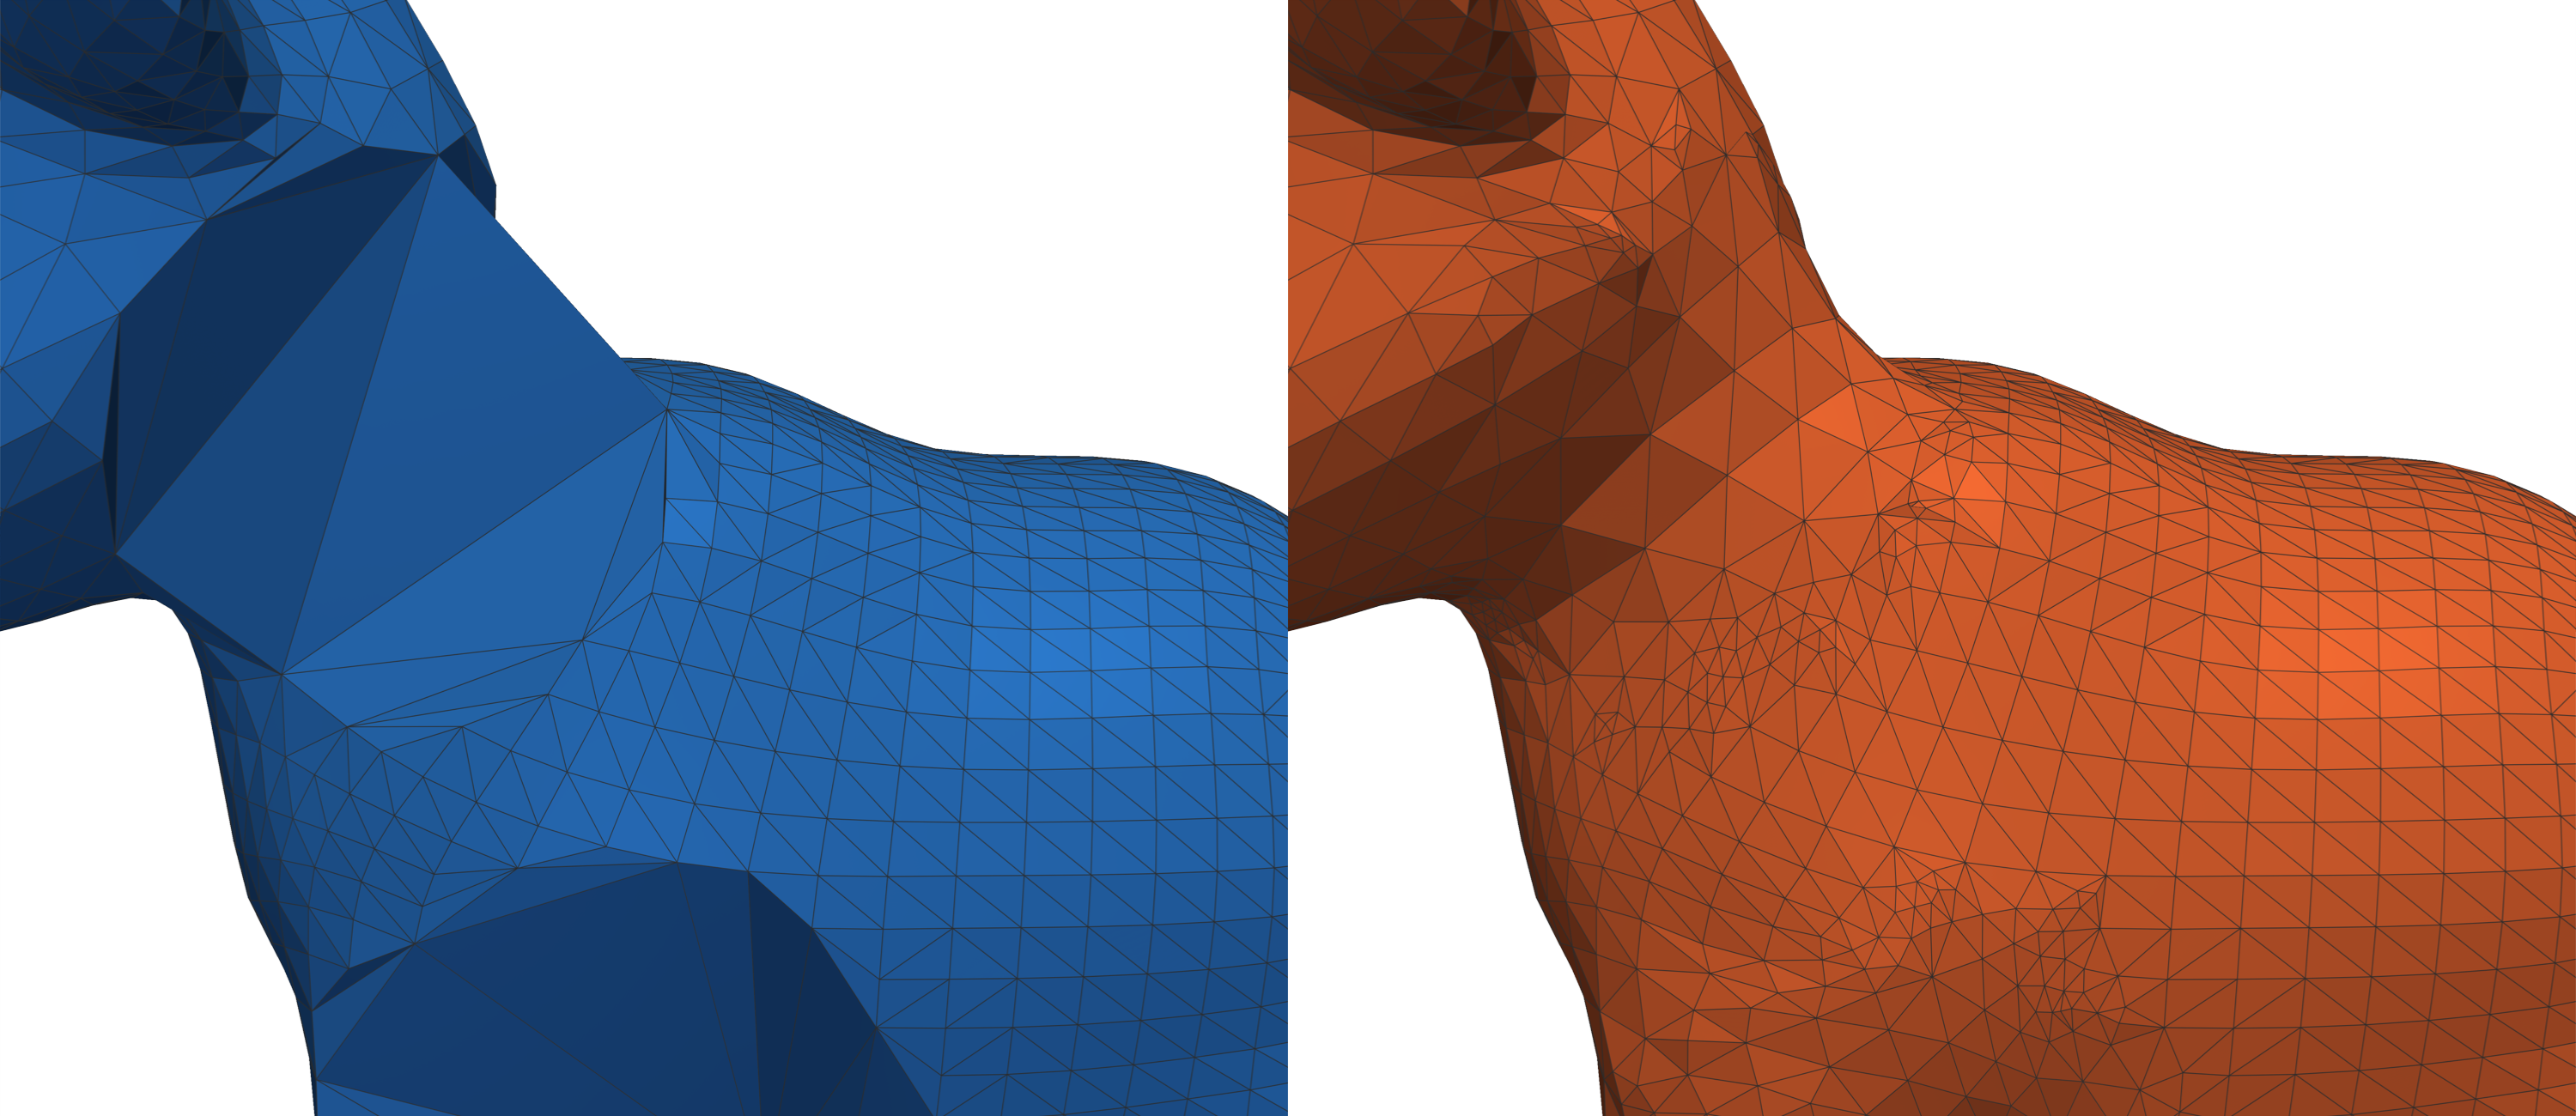
\includegraphics[height=60mm]{figures/cap.png}\par
    {\tinytext\collabel{69mm}{method}{method of [1]}\collabel{69mm}{faired}{with fairing}\par}
    \vspace{3mm}
    {\smalltext\color{ink2}
     \textcolor{faired}{\bfseries Fairing.} The input stays fixed and the cap solves
     \(\Delta^3 x = 0\) [4], which continues it in position, tangent and curvature.\par}
  \end{minipage}\hfill
  \begin{minipage}[t]{150mm}\resetspaces\raggedright
    \centering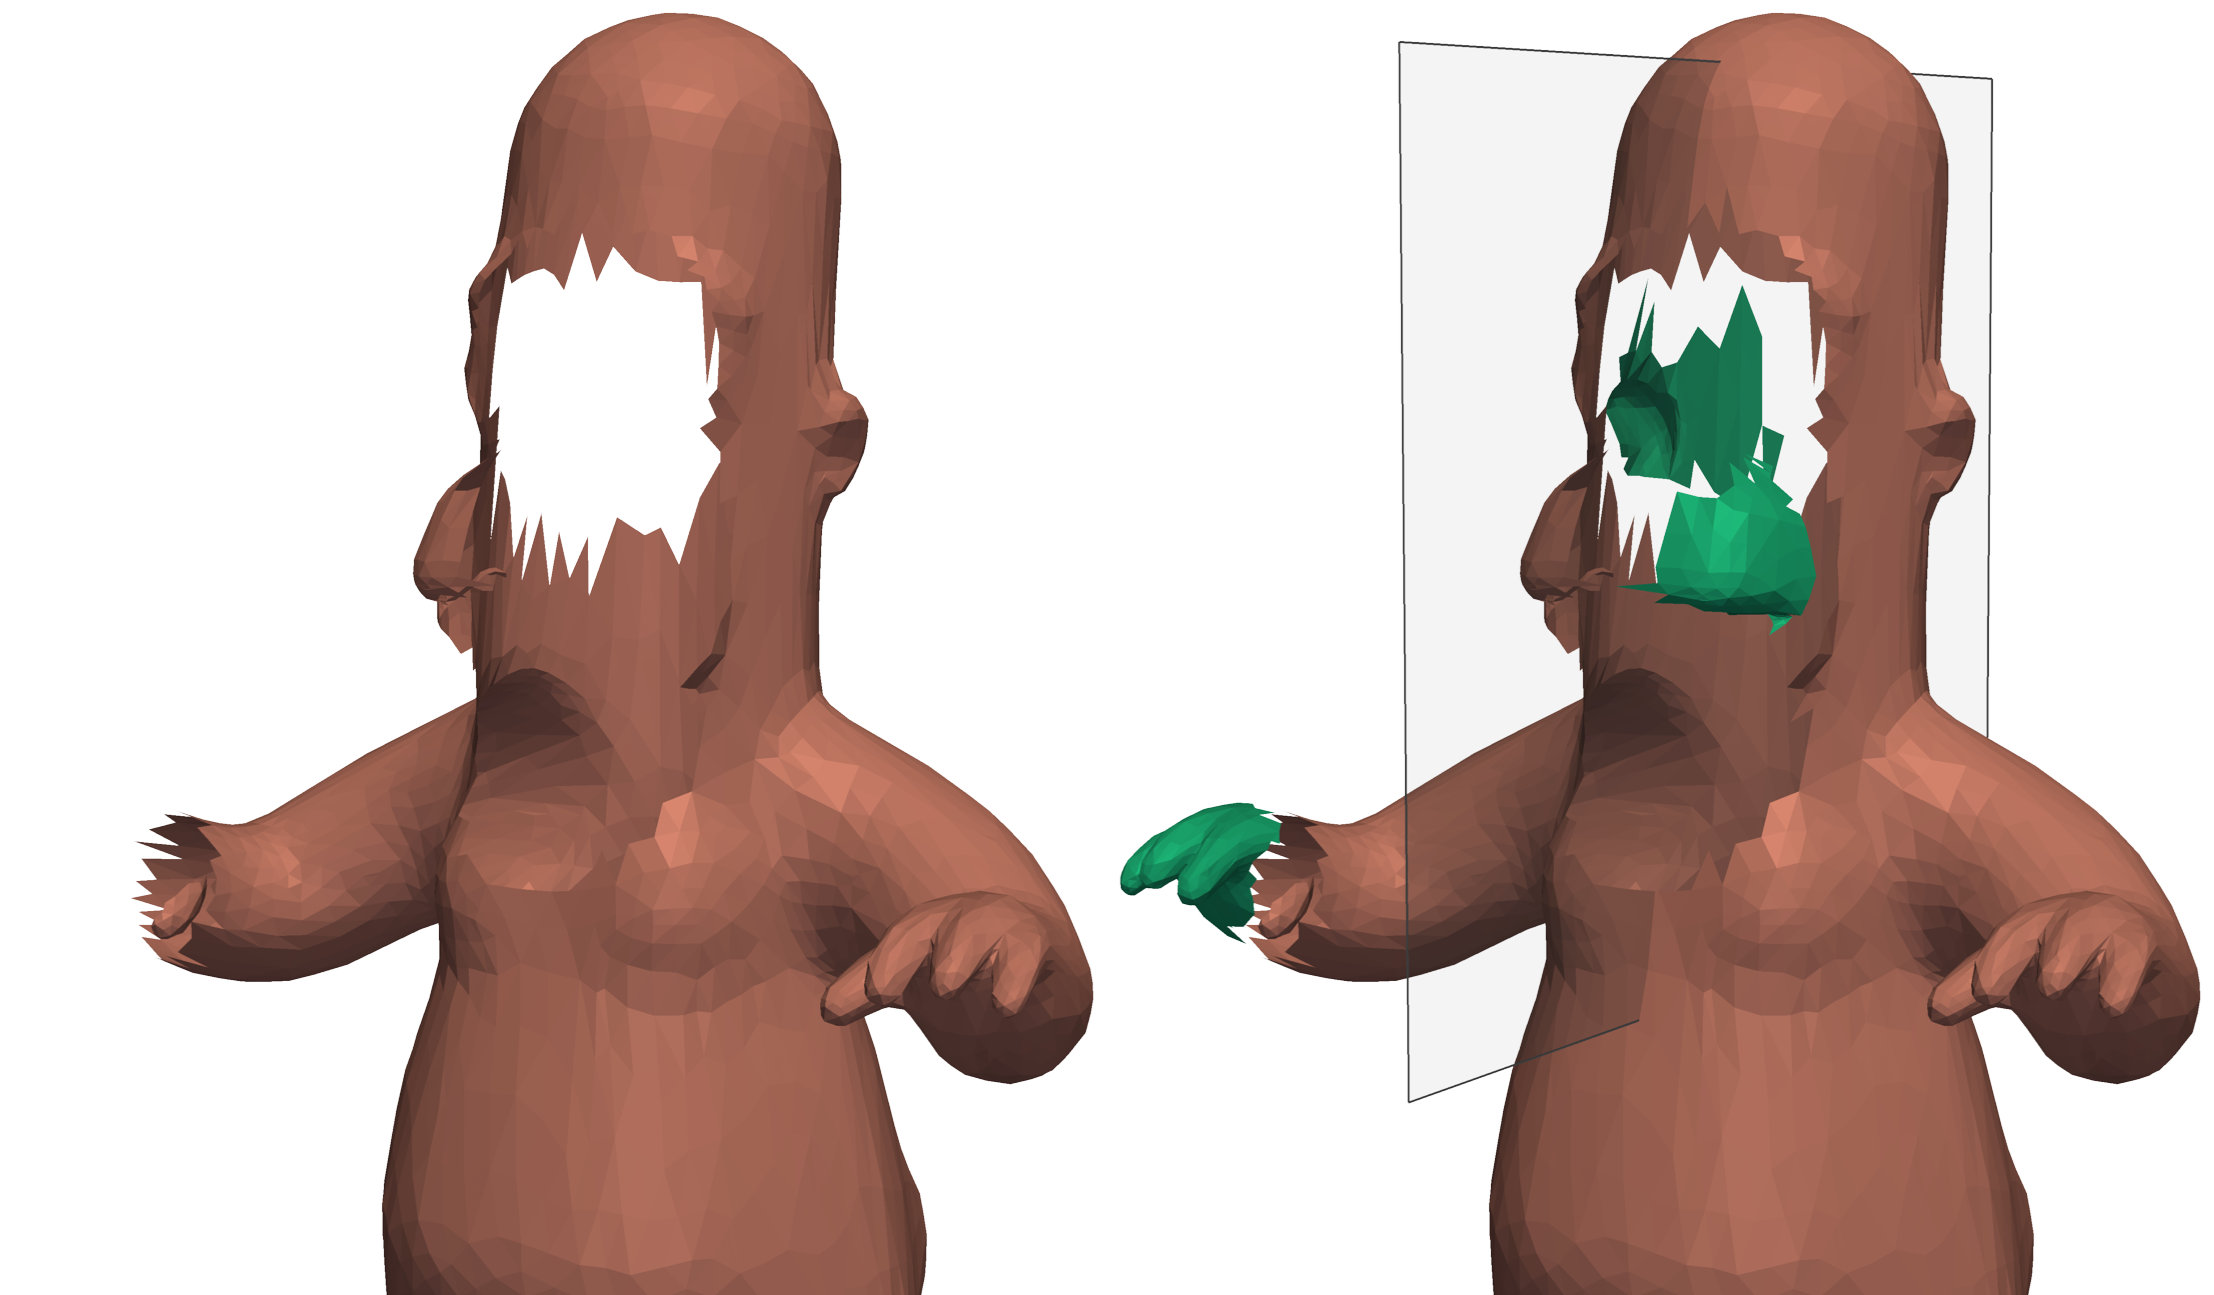
\includegraphics[height=60mm]{figures/mirror.png}\par
    {\tinytext\collabel{51mm}{input}{input}\collabel{51mm}{symmetry}{mirrored faces}\par}
    \vspace{3mm}\raggedright
    {\smalltext\color{ink2}
     \textcolor{symmetry}{\bfseries Symmetry.} The symmetry plane is estimated, and the
     mirrored faces that fall in the holes are added.\par}
  \end{minipage}}

% ---------------------------------------------------------------- 3
\placeblock{25}{581}{650}{\heading{3}{Results}}
\placeblock{25}{607}{350}{%
  \fontsize{22}{28}\selectfont
  \collabel{70mm}{input}{Input}\collabel{70mm}{method}{Method of [1]}%
  \collabel{70mm}{faired}{With fairing}\collabel{70mm}{symmetry}{With symmetry}%
  \collabel{70mm}{original}{Original}\par
  \vspace{3mm}
  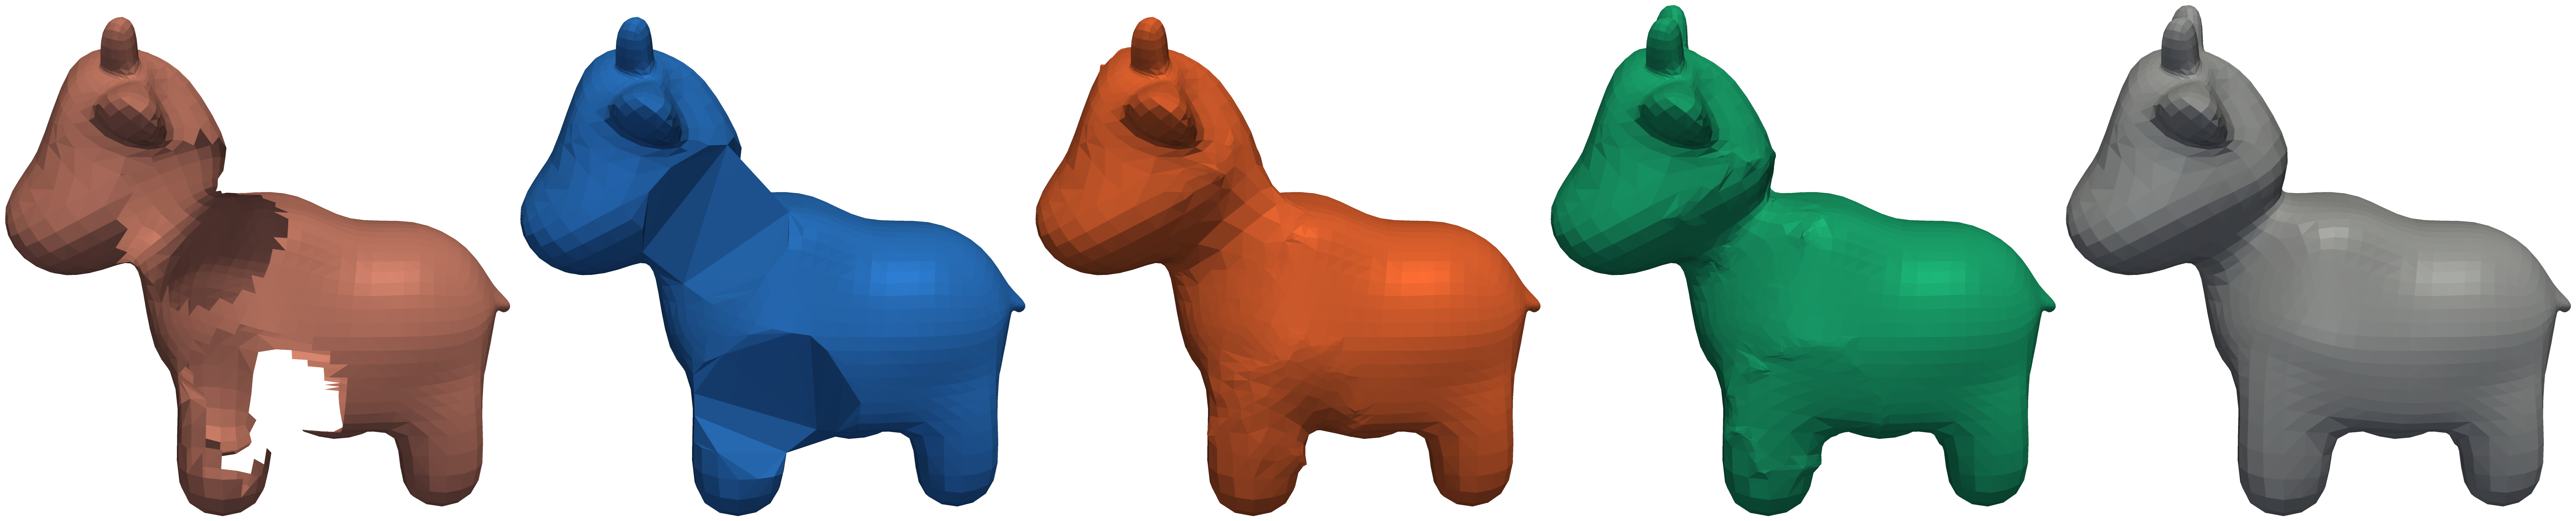
\includegraphics[width=350mm]{figures/spot_22.png}\par
  \vspace{6mm}
  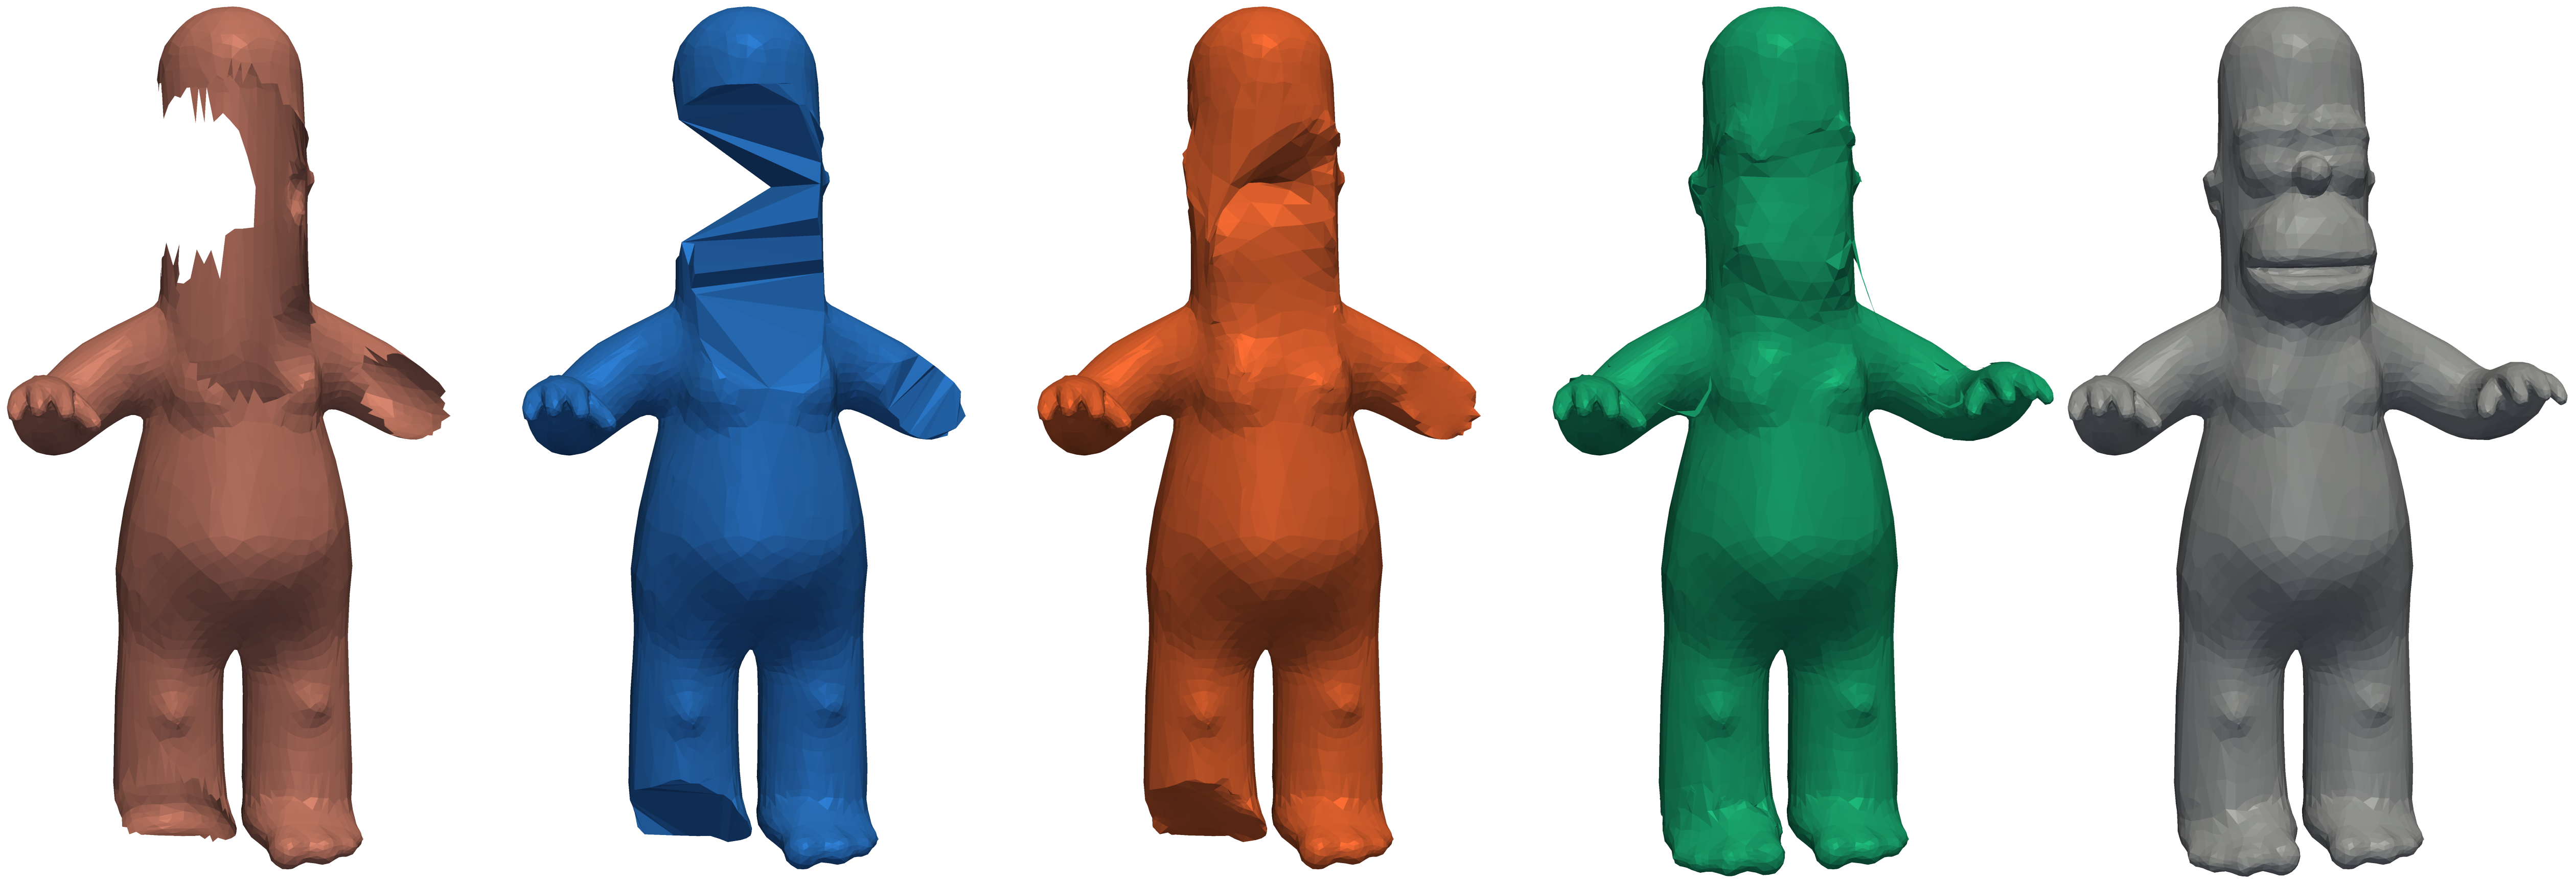
\includegraphics[width=350mm]{figures/homer_22.png}\par}
\placeblock{390}{611}{285}{%
  \begin{minipage}[t]{136mm}\resetspaces\raggedright
    {\fontsize{84}{88}\selectfont\bfseries\color{faired} −43\%\par}
    \vspace{2mm}
    {\smalltext mean error in the holes with fairing. It improves all 18 cases.\par}
  \end{minipage}\hfill
  \begin{minipage}[t]{136mm}\resetspaces\raggedright
    {\fontsize{84}{88}\selectfont\bfseries\color{symmetry} −79\%\par}
    \vspace{2mm}
    {\smalltext with fairing and symmetry. It also improves all 18 cases.\par}
  \end{minipage}\par
  \vspace{5mm}
  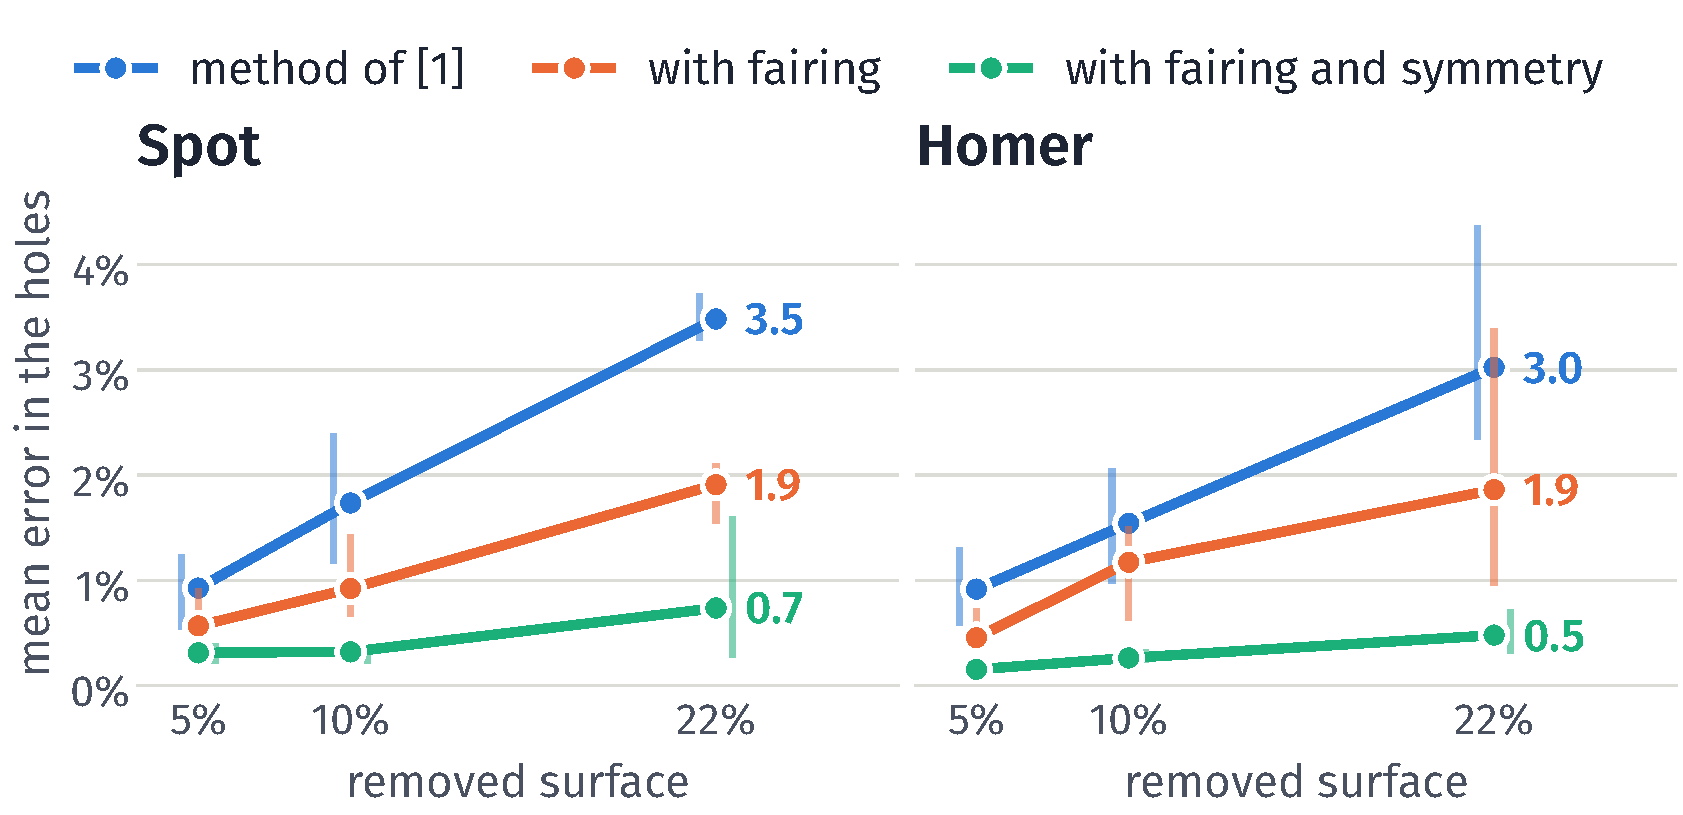
\includegraphics[width=285mm]{figures/error.pdf}\par}

% ---------------------------------------------------------------- 4, 5 and 6
\draw[rule, line width=0.8mm] ($(current page.north west) + (25mm, -835mm)$) -- ++(650mm, 0);
\placeblock{25}{845}{196}{%
  \heading{4}{Limitations}
  \smalltext
  \bulletitem{Symmetry requires a symmetric model whose other side is intact. If surface is
    missing on both sides of the plane, as with the face of Homer at 22\%, there is nothing to
    copy from.}
  \bulletitem{Without symmetry, fairing completes the overall shape but not the small details.}
  \bulletitem{A piece that a hole separates from the rest stays separated, because the cut
    does not control the topology.}}
\placeblock{243}{845}{206}{%
  \heading{5}{Conclusions}
  \smalltext
  \bulletitem{The method of [1] decides correctly what is inside, but it does not give shape
    to what is missing. A local fairing of the caps, which does not move the input, reduces
    the error by 43\%.}
  \bulletitem{Symmetry restores details that fairing cannot invent, such as the face and the
    hand of Homer.}
  \bulletitem{Future work includes partial symmetries, by parts of the model, and a graph cut
    that controls the topology.}}
\placeblock{471}{845}{204}{%
  \heading{6}{References}
  \tinytext
  \bib{1}A.~Jacobson, L.~Kavan, O.~Sorkine-Hornung. Robust inside-outside segmentation using
  generalized winding numbers. \emph{ACM TOG} 32(4), 2013.\par
  \bib{2}H.~Si. TetGen, a Delaunay-based quality tetrahedral mesh generator. \emph{ACM TOMS}
  41(2), 2015.\par
  \bib{3}Y.~Hu et al. Tetrahedral meshing in the wild. \emph{ACM TOG} 37(4), 2018.\par
  \bib{4}M.~Botsch, L.~Kobbelt. An intuitive framework for real-time freeform modeling.
  \emph{ACM TOG} 23(3), 2004.\par
  \bib{5}X.~Li et al. Symmetry and template guided completion of damaged skulls.
  \emph{Computers \& Graphics} 35(4), 2011.\par\vspace{2mm}
  \begin{minipage}[b]{172mm}\resetspaces\raggedright
    Models: Spot (K.~Crane) and Homer (common-3d-test-models). Images and measurements by
    the author.
  \end{minipage}\hfill
  \qrcode[height=27mm]{https://github.com/Lucas-Allara/Broken-mesh-completion}\par}

\end{tikzpicture}
\end{document}
